\documentclass[times, twoside]{zHenriquesLab-StyleBioRxiv}
\usepackage{wrapfig}
\usepackage{graphicx}
% Please give the surname of the lead author for the running footer
\leadauthor{Initiation To Research Project} 

\begin{document}

\title{Measuring the research performance of authors by tacking publishing journals impact factors into account}
\shorttitle{}

\author{Gatien CONTINSOUZAS, Syphax BASSAID, Quentin BROCARD, Mohand BENHADDAD}


\affil[1]{Computer science and statistics Master, Lyon Lumiere University  -Lyon 2- Institute of communication (ICOM), Bron, Lyon, France}

\maketitle

%TC:break Abstract
%the command above serves to have a word count for the abstract
\section*{Abstract}
This paper introduces a new way to calculate the ranking-index for a researcher based on the impact factor of the publishing journal of their research article where each research paper have potentially a specific impact (quality) also based on the journal its published in.\\
This article shows new method to calculate author ranking level metric that measures the quality of a researcher work using the impact of the publishing journals avoiding the h-index which prove it limitation through time.   


\subsection*{Keywords}
h-index, persistence of articles, Graph DBLP, author coefficient

\subsection*{Link}
https://github.com/LariXii/InitRecherche\cite{larix}

\section*{Introduction} 
Research performance evaluation always plays a very important role in scientific development, providing benchmarks for recruitment, promotion, funding, and rewards. To make research evaluation scientific and reasonable, various bibliometric indexes are successively proposed.
However, each indicator has inherent limitations in measuring authors’ research performance \cite{agarwal2016bibliometrics}. These limitations make it challenging to search out the acceptable indicator within the practice of research evaluation and even cause the abuse of bibliometric indicators, or they create the measurement results inconsistent with the particular situation. Therefore, it is necessary to explore the constraints of bibliometric indexes to improve research performance evaluation; particularly, it is important to properly understand a way to use such indexes and how to interpret the measurement results.\\

Based on theoretical and empirical analysis, this paper discusses the limitations of the h-index, and show how other factors influence the quality of a research article. We use DBLP (Digital Bibliography and Library Project) Data base for our experimentation.\\

Hirsch proposed the h-index \cite{hirsch2005index} supported the hypothesis that the quantity of citations a scientist receives reflects the relevance of his/her work over the quantity of papers that he/she publishes. Egghe \cite{egghe2006theory} proposed the g-index in a trial to change or avoid some limitations of the h-index.Subsequently, conducting an in-depth study of the h-index, Prathap \cite{prathap2010there} proposed the p-index, which reveals the arithmetic relationship between the h-index and therefore the number of papers and citations.\\

Although the follow-up indicators noted above were proposed to enhance research evaluation, each indicator has inherent limitations.

\section*{Relative works}
The initial performance evaluation of authors was based on the number of published paper, which essentially measured productivity \cite{agarwal2016bibliometrics}, With the establishment of Garfield's scientific citation index (SCI) system, the frequency of citation was the proxy index of academic influence. However, both measures can reflect only one aspect of research performance evaluation. Laer, Hirsch \cite{hirsch2005index} proposed the h-index, which has attracted increasing attention from researchers because of its robustness and simplicity.\\

Although the h-index was initially proposed as a proxy for the number of citation, it combined the number of paper ans citation. It has also been widely used in the performance evaluation of authors. Hirsch himself \cite{hirsch2005index} recommended the guidelines of h > 12 at a minimum for the promotion of a physicist at a leading university to associate professor and h > 18 for promotion to full professor.\\

Although it is widely used, the h-index has some limitations, such as the incomparability between disciplines, the fact that low-cited and zero-cited papers are ignored, and its insensitivity to papers with a high number of citations. Therefore, many h-type indexes have been proposed to overcome the shortcomings of the h-index.\\

Many indexes have been proposed to eliminate the impact of author cooperation and disciplinary differences. Batista et al. \cite{batista2006possible} divided the h-index by the average number of authors in h papers and designed the $h_{I}$ index. Sidiropoulos et al. used the $h_{f}$ index to obtain the normalized h-index, which aimed to achieve a direct comparison between different subjects \cite{sidiropoulos2007generalized}. Given the shortcomings of the $h_{I}$ index, Schreiber \cite{schreiber2008share} proposed the $h_{m}$ index, which eliminated the defect of the $h_{I}$ index of excessively reducing the influence of large-scale cooperative papers and increasing the influence of individually authored papers an so on.\\
Though the literature review, we think the basic questions of h-index are as follows. The h-index is insensitive to highly cited papers; the h-index value only increases and does not decrease over time; the degree of discrimination for the h-index is low; the h-index ignores most citations and papers outside the h-core. So in our article we will define a new factor that acts about the quality and persistence of a research and we will represent that using graphs.  

\section*{Main Work}
The Digital Bibliography and Library Project (DBLP) is a website publishing a catalog of computer science bibliographies. Hosted by the University of Trier in Rhineland-Palatinate, Germany, it has existed since the 1980s. It was originally conceived as a catalog of bibliographies on databases and logic programming. In January 2015, DBLP lists more than 2.9 million articles on computer science research \cite{dbpl}. Using the xml file shared in the web site we succeed to represent a sample of the data in a graph form containing different information about the possible research paper included in the database as shown in the following figure ( fig : \ref{fig:computerNo0} ). \begin{figure}[h]
\centering
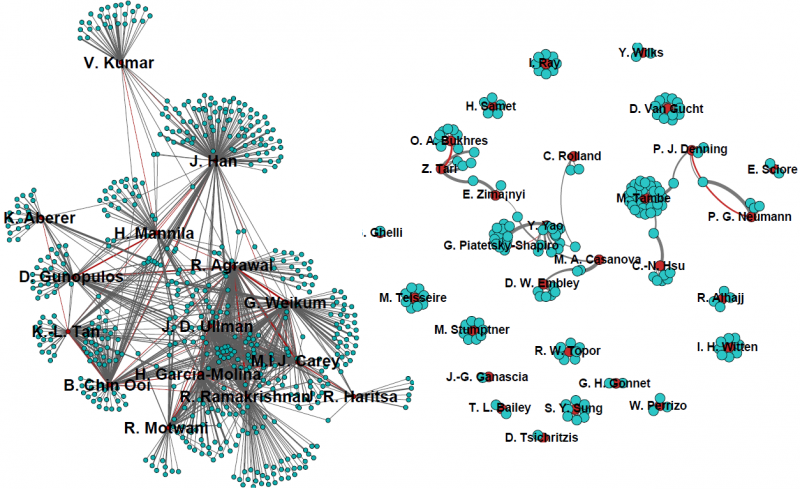
\includegraphics[width=.8\linewidth]{Figures/Figure_1}
\caption{Sample of DBLP graph.}
\label{fig:computerNo0}
\end{figure}
\\The graph presented in this way shows notably some problems by its complexity in terms of description of the data but also by the weak heterogeneity that presents the nodes of the graph. This is due to the incomplete data provided by the DBLP database. We can note the absence of the publishing journals for some articles as well as the h index for all the authors present in the database, this is why that we decided to take only a working sample with complete data to then do manipulations according to the impact factor of the publication journals;\\
The impact factor is a measure of the frequency with which the average article in a journal has been cited in a particular year. It is used to measure the importance or rank of a journal by calculating the times it's articles are cited, this index in generally present in the website of the publishing journals and get updated every year. In our study, after pilling up the right nodes with the complete information, we could obtain the following graph as a result ( fig : \ref{fig:computerNo1} ):
\\
\begin{figure}[h]
\centering
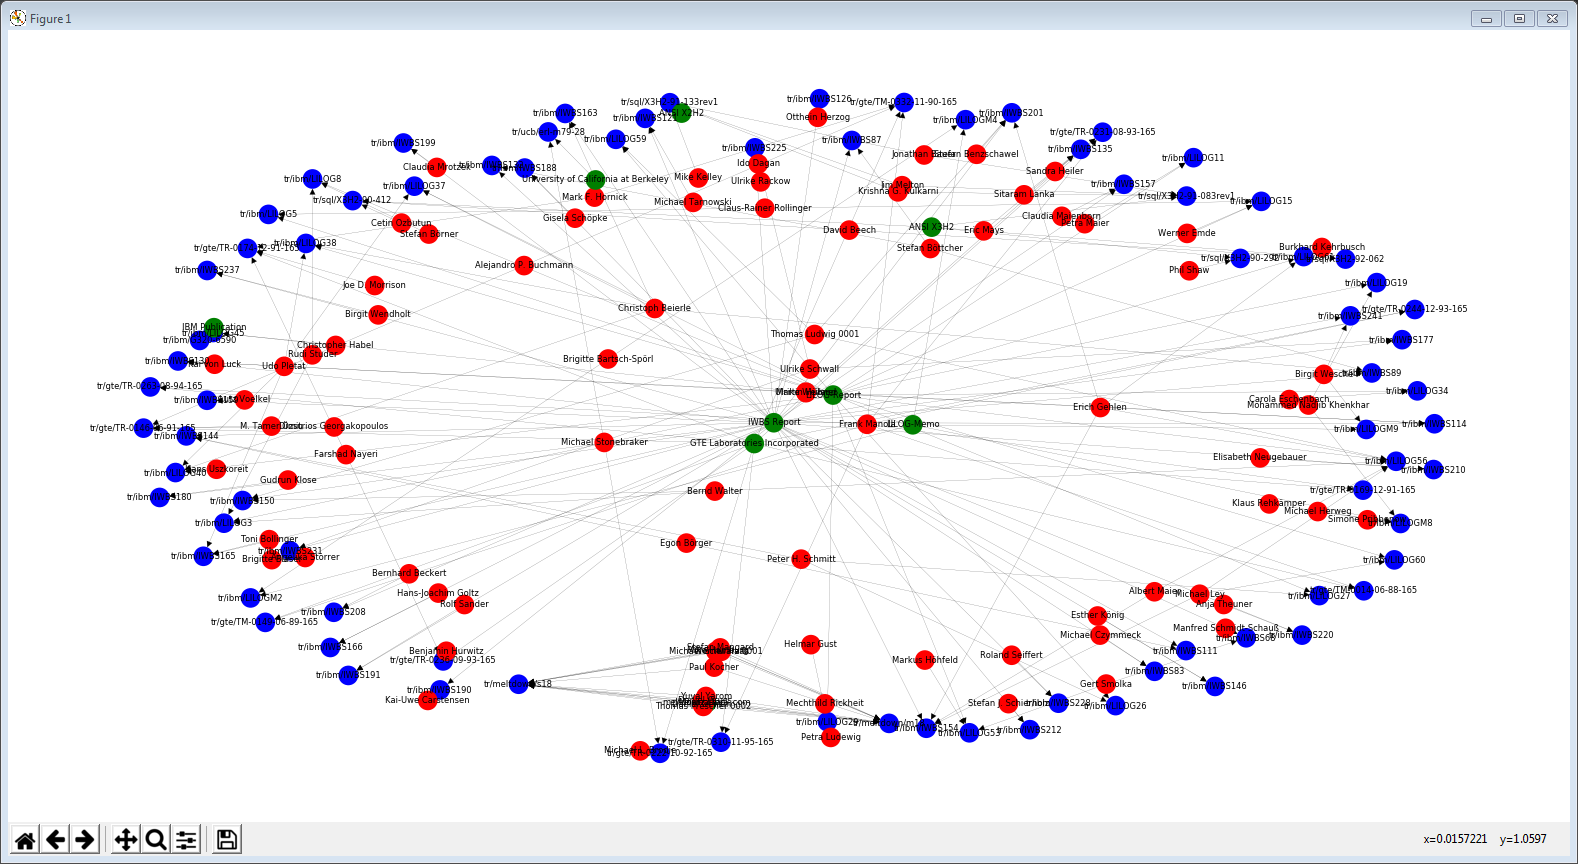
\includegraphics[width=.8\linewidth]{Figures/Graph_1.png}
\caption{Sample of 80 articles from DBLP database.}
\label{fig:computerNo1}
\end{figure}
\\
As Shown in the figure, we notice the presence of three types of nodes with different colors; the "red" refers to \textbf{Authors}, while the "blue" represent the \textbf{Articles} the present authors made, the green nodes in the center of the graph shows the \textbf{publishing journals}.\\
The collection is made by selecting eighty random articles existing in the DB. This selection consist a well choice as a sample for tests, this method is not suitable because of the absence of the impact factor of journals publishing these articles.

Although the work focus on the articles, the right decision is to make a sample based on the publishing journals with explicit impact factors and then to focus on ten of random articles from this publishing journals, that's what obtain in this graph ( fig : \ref{fig:computerNo2} ).\\

\begin{figure}[h]
\centering
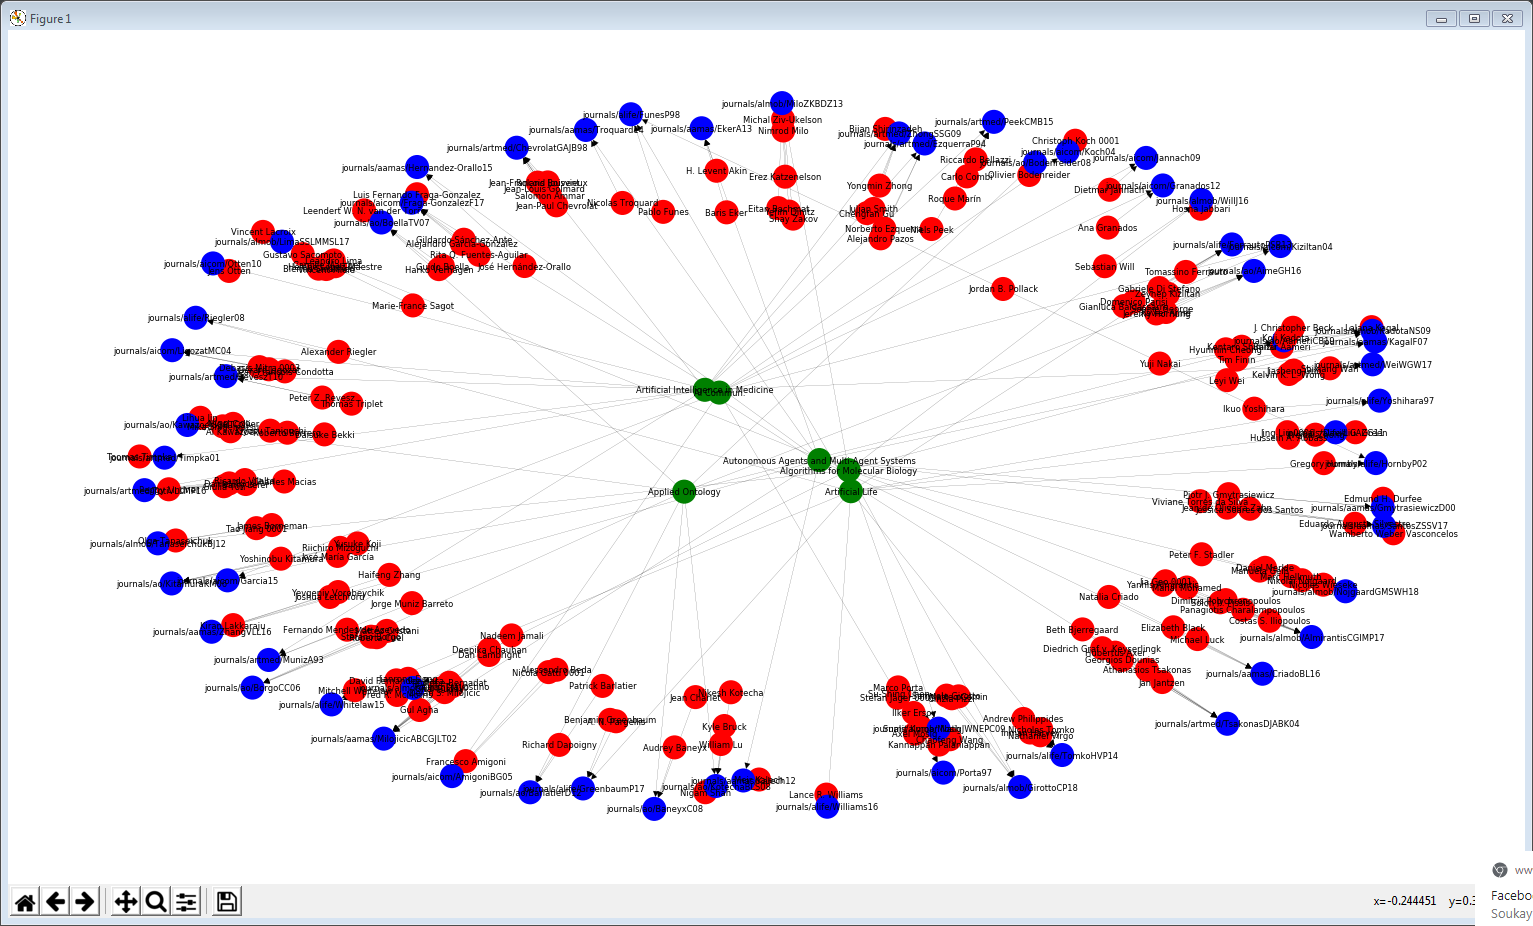
\includegraphics[width=.8\linewidth]{Figures/Graph_2.png}
\caption{Collection of journals with high impact factor.}
\label{fig:computerNo2}
\end{figure}

The graph ( fig : \ref{fig:computerNo2} ) is been significant after collecting interesting publishing journals. the next step is to use a simple formula calculating the coefficient of authors based on the impact of their research article. Generally, the quality of article is linked to the publishing journals they are written and that include this formula :\\
\begin{center}
 $
    X_{a} = \mu (A)_{a} /\sum (A)_{a}
$
\end{center}
Where  $X$ is the authors' coefficient $a$ calculating by the mean of his written article $\mu (A)$ divided per the sum of all his research article $\sum (A)_{a}$ as shown in the graph ( fig : \ref{fig:computerNo3} )
\begin{figure}[h]
\centering
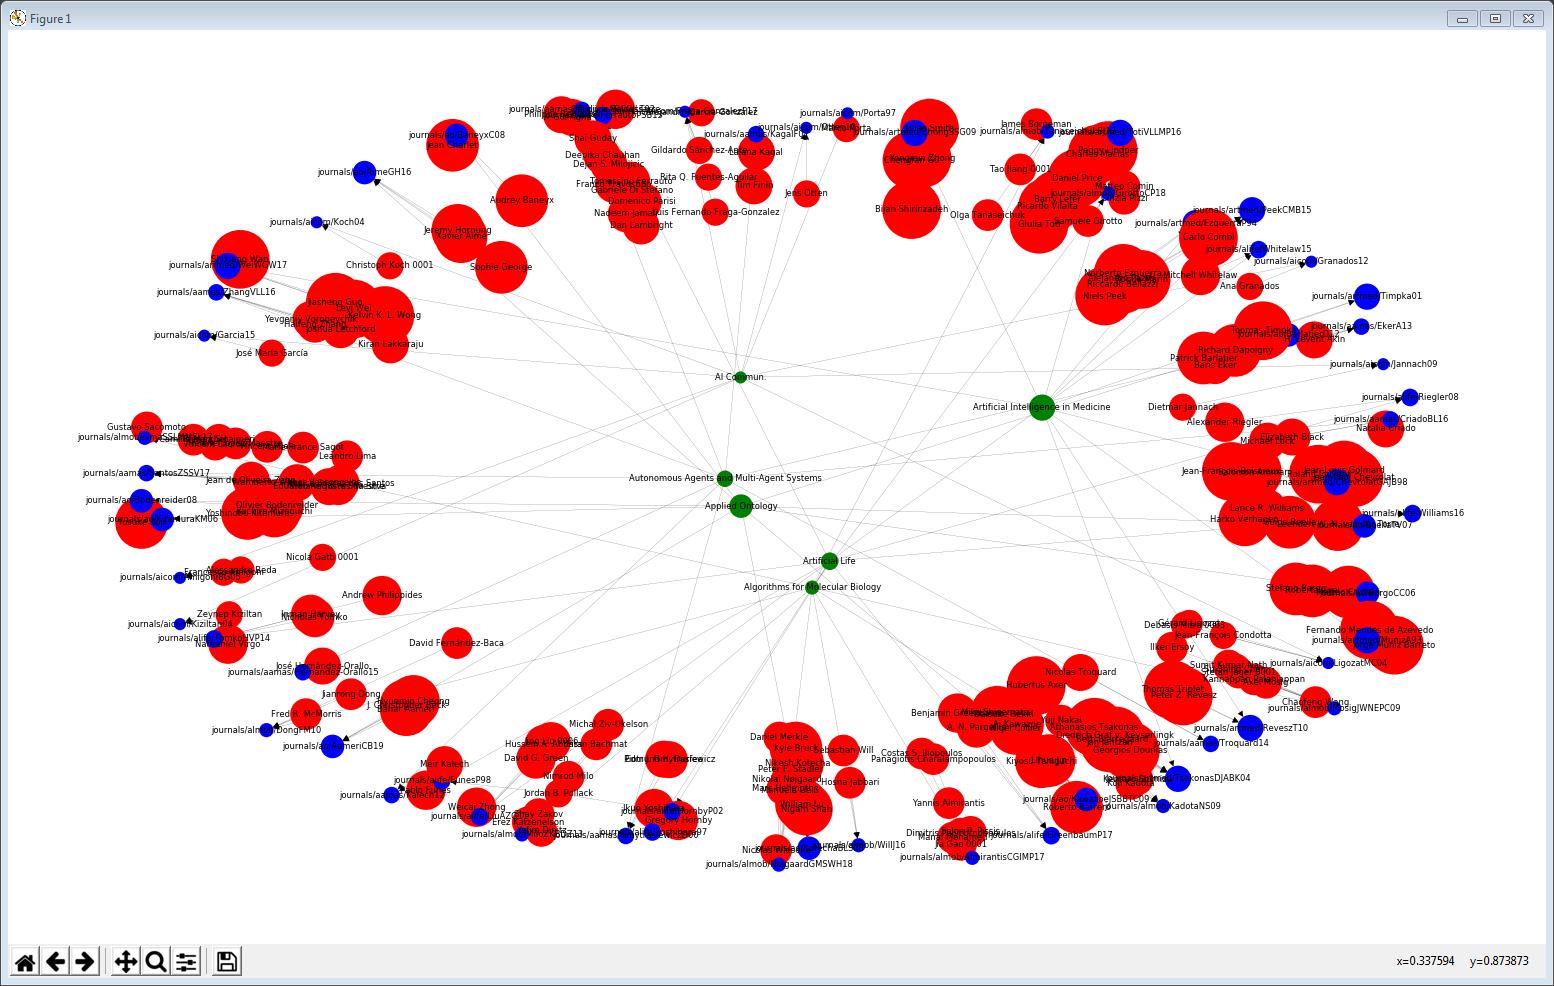
\includegraphics[width=.8\linewidth]{Figures/Graph_dernier.png}
\caption{Scientific journals impact on authors' coefficients.}
\label{fig:computerNo3}
\end{figure}
\\

The distinction is visible and we can effectively tell by looking the "red" nodes referring to article authors' that the quality of an article is mostly linked to the journal that publishes the research and that our study prove that Hirsh-index \cite{hirsch2005index} can be evolve to a more precise index taking other factor into account. In that way, researchers have to "try" to publish in journals with high impact factor, but that is only if the research subject is consistent.

\section*{Conclusions}

Ranking researchers using the h index is an effective but not sufficient way to value a typical researcher or a work (research article) at fair value. In our work, we proceeded by means of graph to calculate a new index by taking as factor the editors of articles.\\This indicates to us that the authors have more impact when the editor of their research work is well classified, either A + rank.\\

We used the DBLP database grouping the majority of research work related to the computer field. Thus including all the authors and the journals of publication as well as the publishers and the years of publication. After cleaning the data, we noted the lack of some information relating to certain work from which we were forced to delete, but also the lack of h-index for each researchers also penalize our search but this was not an obstacle.\\

The visualization of evolution of the researchers h-index compared to the published articles pushed us to base our current research on the factors influencing this index while taking into consideration the studies already made in this field to bring another factor which originally "boost" the impact on the quality of research and our results shows us that the "journal publisher" of research work plays a considerable role and impact on the quality of research work.\\

Although our work can be summed up on only a few factors, this implies that the h index cannot be a sufficient reference for the classification of researchers.
\section*{References}
1. Github code link. https://github.com/LariXii/
InitRecherche. Accessed: 2020-03-25.\\
2. Ashok Agarwal, Damayanthi Durairajanayagam, Sindhuja
Tatagari, Sandro C Esteves, Avi Harlev, Ralf
Henkel, Shubhadeep Roychoudhury, Sheryl Homa,
Nicolás Garrido Puchalt, Ranjith Ramasamy, et al. Bibliometrics:
tracking research impact by selecting the appropriate
metrics. Asian journal of andrology, 18(2):296,
2016.\\
3. Jorge E Hirsch. An index to quantify an individual’s
scientific research output. Proceedings of the National
academy of Sciences, 102(46):16569–16572, 2005.\\
4. Leo Egghe. Theory and practise of the g-index. Scientometrics,
69(1):131–152, 2006.\\
5. Gangan Prathap. Is there a place for a mock h-index?
Scientometrics, 84(1):153–165, 2010.\\
6. Pablo D Batista, Mônica G Campiteli, and Osame Kinouchi.
Is it possible to compare researchers with different
scientific interests? Scientometrics, 68(1):179–189,
2006.\\
7. Antonis Sidiropoulos, Dimitrios Katsaros, and Yannis
Manolopoulos. Generalized hirsch h-index for disclosing
latent facts in citation networks. Scientometrics, 72
(2):253–280, 2007.\\
8. Michael Schreiber. To share the fame in a fair way, hm
modifies h for multi-authored manuscripts. New Journal
of Physics, 10(4):040201, 2008.\\
9. Digital bibliography library project. https:
//fr.wikipedia.org/wiki/Digital_
Bibliography_%26_Library_Project#cite_
note-dblp-1. Accessed: 2020-03-20.
\\
\section*{Biography}
\begin{wrapfigure}{l}{25mm}
\begin{center}
    
\includegraphics[width=1in, hight=1.50in,clip]{Figures/Gatien.jpg}
\end{center}
\end{wrapfigure}\par
  \textbf{Gatien CONTINSOUZAS} is a Computer Science and Statistics Student at Lyon Lumiere University in Lyon -France-. With a Statistics background, he mostly works in this field and does research in this area, he intends to join the OPSIE Master next year in his high degree level.
  \newline
  
  \begin{wrapfigure}{l}{25mm}
  \begin{center}
    
\includegraphics[width=1in, hight=1.50in,clip]{Figures/Syphax.png}
      \end{center}
\end{wrapfigure}\par
  \textbf{Syphax BASSAID} is a Computer Science and Statistics Student at Lyon Lumiere University in Lyon -France- With a background in Networks and Embedded Systems, he joined the research team as handyman whether its in development or in idea giver. He Chooses an OPSIE Master for his last university degree next year. 
 \newline
  
   \begin{wrapfigure}{l}{25mm}
  \begin{center}
    
\includegraphics[width=1in, hight=1.50in,clip]{Figures/Quentin.jpg}
      \end{center}
\end{wrapfigure}\par
  \textbf{Quentin BROCARD} is a Computer Science and Statistics Student at Lyon Lumiere University in Lyon -France-. Comes from a BTS formation, He mostly works as a programmer in research team and help to solves complicated problems linked to programming. Intends to follow an OPSIE Master in the same university he's studying now.
  \newline
  
 \begin{wrapfigure}{l}{25mm}
  \begin{center}
    
\includegraphics[width=1in, hight=1.50in,clip]{Figures/Mohand.JPG}
      \end{center}
\end{wrapfigure}\par
  \textbf{Mohand BENHADDAD} is a Computer Science and Statistics Student at Lyon Lumiere University in Lyon -France-. Already Master degree specialized in Networks and Distributed Systems, and old member in the research center (CDTA) in Algeria, He is preparing a new Diploma in Cyber-Security.


\newpage
\null
\newpage
\bibliographystyle{unsrt}
\bibliography{bibliotheque.bib}
\end{document}



